% !TEX root=/home/tavant/these/manuscript/src/manuscript.tex

\section{Presentation of the Axial-azimuthal simulation}

The objectives of the axial-azimuthal simulation is to allows the azimuthal \ac{ECDI} to grow and study the impacts of the axial direction.
These impacts are mostly due to the radial magnetic field  that present a maximum close to the exit plane.

\subsection{Description of the simulation domaine} \label{subsec-ztheta_description}
\Cref{fig-3Dschematic} shows the simplified \ac{HET} annular channel with both the radial-azimuthal and the axial-azimuthal \ztheta domain.

\begin{figure}[hbt]
  \centering
  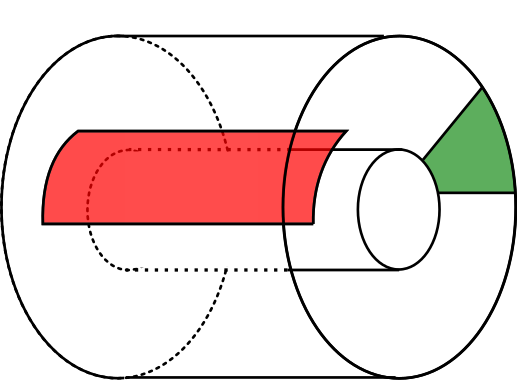
\includegraphics[width=0.6\textwidth]{3D_shematic}
  \caption{Schematic representation of the chamber of a \ac{HET} and (green) the Radial-azimuthal and (red) the axial-azimuthal 2D simulation domains.}
  \label{fig-3Dschematic}
\end{figure}

The \ac{2D} \ztheta domain is located at the mean radius of the channel, but its curvature is neglected.
\Cref{fig-2D_ztheta_bis} presents a schematic representation of the \ztheta simulation domain.
The anode side is closed by a metallic fully absorbing electrode, with a fixed non-zero potential.
On the other side of the domain, the near-plume region (a few centimetres from the exit plane) is modeled.
The boundary located in the near-plume is also a Dirichlet boundary condition, this time grounded.
The azimuthal direction is closed with periodic boundaries for both the particles and the fields.

\begin{figure}[hbt]
  \centering
  \includegraphics[width=0.6\textwidth]{2D_ztheta}
  \caption{Schematic representation of the \ac{2D} \ztheta simulation domain.}
  \label{fig-2D_ztheta_bis}
\end{figure}

The axial and azimuthal electric fields are self-consistently computed from the charge density by solving the Poisson equation.
Consequently, the simulation domain is not so different from the radial-azimuthal simulation domain.
This has allow us to adapt the code \LPPic to simulate both domain.

Two particular aspects have been developed\string: the cathode electron emission and the dynamic computational load balancing.

\paragraph{Cathode electron emission\\}
The cathode used in electrical propulsion are mostly used to neutralize the ion beam, but a significant fraction of the emitted elections enters the channel and travels toward the anode.
The electrons are injected at (or close to) the cathode boundary following a Maxwellian distribution of a few electron volts.
The number of electrons to inject at each time step is computed by closing the eternal circuit between the anode and the cathode.

In the real set-up, an electric filter is placed between the thruster and the generator \citep{barral2008}, originally placed to protect the power supply against AC current.
While this external circuit can be modeled \citep{verboncoeur1993}, and is susceptible to impact the thruster behavior \citep{barral2008,wei2017}, we neglect it in this study for sake of clarity.
Thus, the cathode current equals the anode current \[ I_a = I_c. \]
The corresponding number of electron to inject in the simulation domain depends whether the electron are injected at the boundary or in the domain. 
Therefore, they are developed in the next section.

\paragraph{Dynamic computational load balancing\\}
The axial profile of the plasma density presents a maximum that can be one order of magnitude higher than the mean plasma density.
Consequently, a static MPI domain decomposition would produce an unbalance in the number of numerical particle per CPU, which results in an under-efficient code.

One possibility is to modify dynamically the weigh of the numerical particle relative to the plasma density, in order to keep a relatively constant number of particle per cell.
This can be done by fissioning (merging) the particles when they are too small, or by slitting them in smaller particles when they are too big \citep{shon2001,teunissen2014}.
However, such algorithm can modify the charge, momentum, or the energy of the system if not done carefully.
In \citet{vranic2015}, the authors present an algorithm to  conserve these quantities.
However, we chose not to implement it because of its error-prone complexity.

Instead, we implemented a dynamic redistribution of the CPU domain, so that every CPU own approximately the same number of particle.
As the density gradient is in the axial direction, we only change the axial size of the CPU domains.



\subsection{Facing the breathing mode} \label{subsec-breathmod}
The breathing mode comes from the coupling between the neutral gas flow and the plasma dynamics, via the ionization.
Under the typical conditions of the \ac{HET}, we observed this oscillation with a slows frequency, around  $10-30$ kHz, and a large amplitude, as the plasma density can change up to one order of magnitude during the oscillation period \citep{barral2003a,barral2009}.
This oscillation is much slower than the \ac{ECDI}, and is present in the totality of the channel.

If these oscillations are not problematic for the fluid or \ac{DK} simulations, they are for \ac{PIC} simulations.
Indeed, the total number of numerical particles is proportional to the plasma density, and a minimal number of particles is required to limit the numerical heating \citep{turner2006}.
Thus, when the mean plasma density oscillates, the number of numerical particles (hence the amount of memory used) can change drastically.
This reduces significantly the performance of the simulation code, and can lead to memory overflow if the memory available is not high enough to store all of the particles during the peak of density  of the oscillation.
The \emph{merging-splitting} of the particles  can be used to reduce the variation of the number of numerical particles, but it is not used for the same reason than discussed above.

In addition to the number of particles, the numerical parameters (time step and cell size) have to be chosen to satisfy the stability criteria during all of the simulation, which also reduces significantly the performance of the simulation. 
This could be overcome by adapting dynamically the mesh and the time step.
However, too few studies of the consequences of the use of merging-splitting and adaptive mesh on the simulation results have been conducted.
Thus, we have chosen not to modify the \ac{PIC} algorithm.


Two other approaches have been followed to reduce the computational cost of the breathing mode\string:
\begin{enumerate}
  \item the approach used by \citet{coche2014}\string: using a scaling of the permittivity to reduce the computational load,
  \item the approach of \citet{boeuf2017}, using a forced ionization source term.
\end{enumerate} 

\paragraph{Coche's simulation case \\}

The simulation proposed by \citet{coche2014} models self-consistently the ionization with the \ac{MCC} algorithm, as well as the neutral gas flow by supposing a constant velocity.
\Cref{fig-coche-presnetation} presents the domain of simulation.
The simulation domain geometry is realistic, with a channel length $L_{channel} = 2.5\,\centi\meter$ for a total axial length of the simulation domain $L_z=4\,\centi\meter$.
Hence, all of the chamber and a part of the near plume is simulated.

\renewcommand\subfigurewidth{0.4\textwidth}


\begin{figure}[hbt]
  \centering
  \begin{tabular}{cc}
    \subfigure{coches_domain}{}{10,10} &
    \subfigure{coches_profiles}{}{10,10} \\
  \end{tabular}
  \caption{(left) the \ac{2D} axial azimuthal domain; (right) the axial profile of the magnetic field and the initial xenon neutral gas profile used for the simulation case of Coche. }
  \label{fig-coche-presnetation}
\end{figure}

The constraints on the time step and the cell size are alleviated by using a scaling on the permittivity.
It is simply increased by a coefficient $\alpha$, as used in other low-temperature modelling \citep{fubiani2012,boeuf2012,liu2010}.
The electron plasma frequency and electron Debye length thus become (starred quantities)
\begin{equation} \label{eq-scaled_lde}
  \lde^* = \sqrt{\frac{\alpha \epsilon_0 \Te}{e n_e}} = \lde \alpha^{1/2}
\end{equation}
\begin{equation} \label{eq-scaled_wpe}
  \ope^* = \sqrt{\frac{e^2 n_e}{\alpha \epsilon_0 m_e}} = \ope \alpha^{-1/2}
\end{equation}
Hence, the constraints on the time step and the cell size are reduced by a factor $\sqrt{\alpha}$
\begin{align*}
  \Delta t ^* &= \alpha^{1/2} \Delta t \\
  \Delta x ^*&= \alpha^{1/2} \Delta x  
\end{align*}

By using a factor $\alpha=80$,  which correspond to a factor of $9$ on the time step and the cell size,  \citet{coche2014} successfully observed the breathing mode in the \ac{PIC}-\ac{MCC} simulation.


\paragraph{Boeuf's simulation case \\}

In \citet{boeuf2018}, the authors used a simplified simulation set-up in order to better study the azimuthal instabilities.
The simulation is collisionless and the ionization profile is not-self-consistent but  is given as an input of the model.
This allows to remove the breathing mode oscillations from the discharge, and to simplify the parametric study of the plasma density.
The simulation domain is also smaller than the usual chamber, reducing again the computational load.



\begin{figure}[hbt]
  \centering
  \begin{tabular}{cc}
    \subfigure{boeuf-domain.png}{}{10,10} &
    \subfigure{boeuf-profiles.png}{}{10,10} \\
  \end{tabular}
  \caption{(left) the \ac{2D} axial azimuthal domain; (right) the axial profile of the magnetic field and the ionization source term profiles used for the simulation case of Boeuf. }
  \label{fig-boeuf-presnetation}
\end{figure}

\inlinenote{The simulation models (boundary conditions and so on) need to be given. See the publications (Thomas' and Boeuf's)}

\subsection{Model for radial losses} \label{subsec-fakeR}

In this section, we discuss the objective to add to the purely \ac{2D} axial-azimuthal \ac{PIC} simulation the impact of the radial walls.
The first effect that we want to model is the particle and power losses to the wall.
Thus, as previously done in the radial-azimuthal simulation, the particles are tracked in the three directions.
A finite radial length is used to limit the radial direction.
To begin with, we do not model the secondary electron emission.

When an ion crosses the boundary, it is removed from the simulation.
The electrons should be reflected by a sheath that results in an electron flux absorbed at the wall equal to the ion flux.
We suppose that the sheath is infinitely thin, so that the wall corresponds to a partially reflecting surface.
Two approaches have been investigated to model efficiently the effect of the sheath.


\paragraph{ Model 1 for the radial losses\string: sheath model\\}
The first approach set the potential drop at the walls by using  a sheath model, such as the one in \cref{sec-sheath}, or in \cref{ch-3,ch-4}.
The ions would be absorbed by the radial boundary, as well as the electrons of energy higher than the sheath potential.
Electrons with smaller energy are reflected spectacularly.

This model is more physical, but it would allow local charge imbalance.
Moreover, as there is no electric field self-consistently computed in the radial direction, the plasma cannot react to such imbalances.
Hence, we chose not to use it.

\paragraph{Model 1 for the  radial losses\string: flux equality\\}
The second approach directly imposes the flux equality by absorbing every time step the same number of electrons as ions.
The electrons crossing the radial boundaries are sorted by their energy, and the electrons absorbed are the most energetic ones.
The others are reflected elastically.
Due to the small number of ions crossing the boundary, and for performance issues, we choose to impose the flux equality averaged over the domain of a CPU.
As 360 CPU domains are used to decompose the whole simulation domain, this allows a partial locality of the flux equality. 
\vspace{1ex}
While the sheath can be supposed infinitely fin, the ion flux to the wall depends on the pre-sheaths, which usually display an ambipolar electric field that accelerates the ions to the ion sound speed at the sheath edge.
Since the development and validation of a pre-sheath electric field in the radial model required more resources than available, there is no such pre-sheath model present in the results presented in this chapter.
Consequently, the ion flux to the wall is a thermal flux, which is much smaller than the flux created by a pre-sheath.
Hence, using a realistic radial length  of the order of 1 or $2\,\centi\meter$, the particle losses are underestimated.
One solution is to reduce the radial length, so that the particle flux are closer to physical losses.

In the results given in the next sections are obtained with modeling the radial losses in all of the simulation domain.
This is done in order not to introduce a discontinuity, as well as to increase the impact of the radial losses on the simulation results.
